\documentclass[a4paper]{article}
\usepackage{url}
\usepackage{INTERSPEECH2020}
\usepackage{cite}
\usepackage{tablefootnote}
\usepackage{color}
\usepackage{graphicx} 
\usepackage{epstopdf, multirow}


\usepackage{pifont}
\usepackage{footnote}
\makesavenoteenv{tabular}
\newcommand{\quotes}[1]{``#1''}
\setlength{\intextsep}{2pt plus 0pt minus 3pt} %distance between floats on the top or the bottom and the text
\setlength{\textfloatsep}{2pt plus 0pt minus 4pt}%distance between two floats
\setlength{\floatsep}{2pt plus 0pt minus 2pt}%distance
\usepackage{soul}
\title{Unsupervised Subword Modeling Using Autoregressive Pretraining and Cross-Lingual Phone-Aware Modeling}
\name{Siyuan Feng, Odette Scharenborg}
%The maximum number of authors in the author list is twenty. If the number of contributing authors is more than twenty, they should be listed in a footnote or in acknowledgement section, as appropriate.
\address{
  Multimedia Computing Group, 
  Delft University of Technology, Delft,  the Netherlands}% \\
 %$^2$Department of Electronic Engineering, The Chinese University of Hong Kong, Hong Kong}
\email{\{s.feng, o.e.scharenborg\}@tudelft.nl}

\begin{document}

\maketitle
% 
\begin{abstract}
This study addresses unsupervised subword modeling, i.e., learning feature representations that can distinguish subword units of a language. 
The proposed approach adopts a two-stage bottleneck feature (BNF) learning framework, consisting of 
autoregressive predictive coding (APC) as a front-end  and a 
% cross-lingual phone-aware 
DNN-BNF model as a back-end. 
APC pretrained features are set as input features to a DNN-BNF model. A  language-mismatched ASR system is used to provide cross-lingual phone labels for DNN-BNF model training. Finally, BNFs are extracted as the subword-discriminative feature representation. A second aim of this work is to investigate the robustness of 
% the proposed 
our
approach's effectiveness to different training data amounts. The results on Libri-light and ZeroSpeech 2017 databases show that APC is effective in front-end feature pretraining.
Our whole system outperforms the state of the art on both databases.
Cross-lingual phone labels for  English data by a Dutch ASR are better than by a Mandarin ASR, possibly linked to the larger similarity of Dutch than Mandarin with English.
% Moreover, 
Our system is less sensitive to training data amount  when the training data is over 50 hours.  
% Concluding, 
APC pretraining leads to a reduction of needed training material from over 5,000 hours to around 200 hours with little performance degradation.


\end{abstract}
\noindent\textbf{Index Terms}: unsupervised subword modeling, autoregressive predictive coding, cross-lingual knowledge transfer

\section{Introduction}

% Automatic speech recognition (ASR) has achieved impressive performance in recent years for major languages such as English \cite{Han2019State,Wang2019Transformer}.
% , thanks to the successful application of deep neural networks (DNNs) in acoustic and language modeling. 
% Acoustic modeling is a core component in building an ASR system. 
% It is   considered a supervised learning problem.  
Training a DNN acoustic model (AM) for a high-performance automatic speech recognition (ASR) system requires a huge amount of speech data paired with  transcriptions. 
%While this is considered not a problem for  languages such as English and Mandarin, 
Many languages in the world have very limited or even no transcribed data \cite{dunbar2017zero}. 
% In an extreme scenario where there are no transcribed data available for the concerned  language, 
% these languages are usually referred to as \textit{low-resource} languages. C
Conventional supervised acoustic modeling techniques are thus problematic or even not applicable to these languages.
% to low-resource languages.

Unsupervised acoustic modeling (UAM) refers to the task of modeling basic acoustic units of a language with only untranscribed speech \cite{chen2015parallel,heck2017feature,Kamper2017segmental,Tjandra2019,Feng2019combining,Ondel2019Bayesian}. %It is  challenging and  with significant research impacts. It has been studied in applications to languages without orthographic transcriptions \cite{I3EWang}, query-by-example spoken term detection \cite{Chen+2016}, text-to-speech without text \cite{Dunbar2019}, topic identification \cite{SiuGishChanEtAl2014}, etc. Unsupervised acoustic modeling could also be applied to documentation of unwritten languages, and understanding infants' language acquisition mechanism \cite{versteegh2015zero}. 
%Recently, there has been an increasing  interest in unsupervised acoustic modeling \cite{chen2015parallel,heck2017feature,Kamper2017segmental,Tjandra2019,Feng2019combining,Ondel2019Bayesian}, which resulted in the Zero Resource Speech Challenges (ZeroSpeech). 
% This is partially driven by Zero Resource Speech Challenges (ZeroSpeech) \cite{versteegh2015zero,dunbar2017zero,Dunbar2019}.
%One  research problem tackled by Zero Resource Speech Challenges (ZeroSpeech) \cite{versteegh2015zero,dunbar2017zero,Dunbar2019}
An important task in UAM is to learn frame-level feature representations that can distinguish subword units of the language for which no transcriptions are available, i.e., the \textit{target} language, and is 
% concerned language and is
robust to non-linguistic factors, such as speaker change \cite{versteegh2015zero,dunbar2017zero}. This problem is referred to as \textit{unsupervised subword modeling}, and is the focus of this study. It is essentially a feature representation learning problem.
% It is essentially an  unsupervised feature   learning problem.
% , it serves as the basis for 

% another widely studied problem in unsupervised acoustic modeling, i.e. discovering a set of basic subword units that could represent a language
%  \cite{Ondel2019Bayesian}. 
%  The present study addresses   unsupervised subword modeling.

There are many interesting attempts  to unsupervised subword modeling \cite{chen2015parallel,heck2017feature,chorowski2019unsupervised,shibata2017composite,feng2019_TASLP,riviere2020unsupervised,Feng2019combining}. One research strand is to use purely unsupervised learning techniques 
% which are effective in subword modeling 
% towards target untranscribed speech data 
\cite{chen2015parallel,heck2017feature,chorowski2019unsupervised}. For instance, Chen et al. \cite{chen2015parallel} proposed a Dirichlet process Gaussian mixture model (DPGMM) posteriorgram approach, which performed the best in ZeroSpeech 2015 \cite{versteegh2015zero}.  Heck et al. extended this approach by applying unsupervised speaker adaptation, which performed the best in ZeroSpeech 2017 \cite{heck2017feature}. 
% Vector quantized variational autoencoder (VQ-VAE) \cite{chorowski2019unsupervised} and factorized hierarchical VAE (FHVAE) \cite{Feng2019improving} were applied 
% {\color{blue}
In a recent study \cite{Feng2019improving}, a two-stage bottleneck feature (BNF) learning framework was proposed.
% investigated. 
The first stage, i.e., the front-end, used the factorized hierarchical variational autoencoder (FHVAE) \cite{hsu2017nips} to learn speaker-invariant features. The second stage, the back-end, consisted of a DNN-BNF model \cite{chen2017multilingual}, which used the FHVAE pretrained features as input features and generated BNFs as the desired subword-discriminative acoustic feature representations. In the case of unsupervised acoustic modeling, no frame labels are available for DNN-BNF model training.
% Frame labels required for DNN-BNF training  are not directly available due to the absence of transcriptions. 
In \cite{Feng2019improving},
 DPGMM was adopted  
%  {\color{blue} 
 as a building block of the back-end
%  } 
 to generate pseudo-phone labels for the speech frames.
%  ,
%  }
In another recent study  \cite{chorowski2019unsupervised}, the vector quantized VAE (VQ-VAE) \cite{oord2017neural} was applied to directly learn the desired feature representation without a back-end model such as the DNN-BNF, and is comparable to state-of-the-art performance \cite{heck2017feature}. 
% {\color{blue}
% In \cite{riviere2020unsupervised}, contrastive predictive coding (CPC) was applied \cite{oord2018cpc}. 
%The performance of \cite{chorowski2019unsupervised} is comparable to state of the art \cite{heck2017feature}.
% They do not require a back-end model for subword discriminative modeling.
% }
% Factorized hierarchical VAE (FHVAE) was applied in \cite{Feng2019improving}. In this work, a 
% Their results are on par with \cite{heck2017feature}.
% , and was further applied in subsequent studies \cite{chen2017multilingual,heck2017feature} with improvements. 

In another research strand, frame-level feature representations that can distinguish subword units in the target language are created using a cross-lingual knowledge transfer approach \cite{feng2019_TASLP,shibata2017composite}. Here, out-of-domain (OOD) mismatched language resources are used to train DNN AMs which are further used to extract phone posteriorgrams or BNFs of the target speech.
% Another research direction is to exploit out-of-domain (OOD) mismatched language resources
% % to model  target zero-resource speech 
% \cite{feng2019_TASLP,shibata2017composite}, in what is essentially a cross-lingual knowledge transfer approach. Here, 
% % {\color{blue} 
% DNN AMs of 
% % } 
% OOD languages are used to extract phone posteriorgram or BNFs of the target speech. 
% {\color{blue}
% }
% as the desired representation.
% in a language-mismatched manner. 
% \cite{feng2019_TASLP} also proposed to OOD ASR systems to % In these studies,  Phonetic and speaker  information from out-of-domain languages were both  
% from out-of-domain resource-rich 
% DNN AMs for a resource-rich language were trained using a transcribed speech corpus, and used  to extract bottleneck features (BNFs) for target speech in a language-mismatched manner.  
The two research strands mentioned above can also be combined.
% to  achieve improved performance. 
For instance, \cite{feng2019_TASLP} proposed to 
% {\color{blue}
apply the DNN-BNF model, and  utilized  unsupervised   DPGMM  and OOD ASR systems  to  generate two types of frame labels for multi-task DNN-BNF learning. The two label types correspond to  the two research strands respectively. 
% The BNFs are extracted by the DNN-BNF model. 
The results  showed the complementarity of the two label types in unsupervised subword modeling.
% that applying two types of labels is superior to applying either one type.
% its superiority over applying either one label type as supervision. 
% The back-end DNN-BNF model is widely applied for the concerned problem \cite{chen2017multilingual,feng2018exploiting,Higuchi2019}.
% , the DNN-BNF is adopted as the back-end for subword-discriminative modeling
% }
% to  i.e. frame labeling followed by DNN-BNF modeling. Two frame label types, i.e., DPGMM clustering labels and OOD ASR labels, are jointly used to train 

% {\color{blue}
The present study  adopts a two-stage BNF learning framework similar to  \cite{Feng2019improving}, and aims at
% }
% aims at 
combining unsupervised   learning techniques, specifically autoregressive predictive coding (APC) as a front-end, with  cross-lingual   knowledge transfer in the back-end. 
% Our proposed approach consists  front-end unsupervised pretraining and back-end DNN-BNF  modeling. 
% The two-stage framework is similar to \cite{Feng2019improving} as mentioned above.
% This two-stage framework is similar to \cite{Feng2019improving} mentioned above.
% In the first stage,  APC  is adopted as the unsupervised learning front-end.
Recently, APC   has   been shown   \cite{Chung2019} to learn speech feature representations that are beneficial to 
% .... and to outperform other unsupervised ....
% was recently proposed \cite{Chung2019} to learn speech feature representation that is beneficial to 
various downstream   tasks, and outperform other effective
% to perform well, as compared to spectral features. 
% It has been shown to outperform other  
unsupervised methods such as contrastive predictive coding (CPC) \cite{oord2018cpc} 
% and problem-agnostic speech encoder (PASE) \cite{Pascual2019} 
in ASR, speech translation and speaker verification   \cite{Chung2019generative}.
% {\color{blue}
 APC preserves   phonetic (subword) and speaker information from the original speech signal, while the two information types are more  separable. This makes APC a possibly interesting  method for unsupervised subword modeling. %,
%   and are more accessible to task-specific back-ends.
% %  }
% While it is not designed exclusively for learning subword-discriminative features, we expect  front-end APC pretraining
% could increase the accessibility of phonetic information   to the  back-end of our adopted framework.
% pretrained features could encode subword information more easily accessible to our back-end modeling. 
In this paper, we investigate the effectiveness of APC in this task for the first time.
% Motivated by this, we, for the first time, propose to apply APC in unsupervised subword modeling.

In  the second stage, a DNN-BNF back-end is trained, using the APC pretrained features as input features. 
% APC pretrained   features 
% and cross-lingual phone labels, obtained based on an OOD ASR system,  
% are used as input features to train a DNN-BNF  back-end. 
Frame labels required for  DNN-BNF model training are obtained using an OOD  ASR system as was done in \cite{feng2019_TASLP}.  
% {\color{blue} 
By doing so, cross-lingual phonetic knowledge is exploited.
% }
% The BNFs are then extracted as the desired subword-discriminative acoustic feature representations. 
% {\color{blue} 
Two OOD ASR systems trained on  different OOD languages are employed for comparison, in order to study the effect of target and OOD language similarity on the performance of the proposed approach.
% }
% The efficacy of cross-lingual frame labeling in unsupervised subword modeling  has been shown by \cite{feng2018exploiting,feng2019_TASLP}. In this study, 
% the effect of APC pretraining in unsupervised subword modeling 
% is investigated  by combining with  DNN-BNF.
% modeling.

% in tackling the unsupervised subword modeling task, 
%  DNN-BNF modeling with cross-lingual labels is
% % cross-lingual phone-aware DNN-BNF is 
% combined  with APC pretraining to achieve further performance improvement.
% in unsupervised subword modeling.
% , where cross-lingual labels are obtained by applying an OOD ASR system.
% an OOD ASR system is applied to assign a phone label for each target untranscribed speech frame.
% of target zero-resource speech. 
% These cross-lingual phone labels and APC pretrained features are used  to train DNN-BNF models. 
% effective Approaches 
% 1. Purely unsupervised approaches
%   1.1 DPGMM
%   1.2. VQ-VAE
% 2. exploiting cross-lingual resources
%   1.1. DNN-BNF with DPGMM labels and cross-lingual phone labels
% for major languages, such as English and Mandarin. One major reason is that 


% untranscribed training data amount.  
For low-resource languages for which transcribed data are absent, 
even unlabeled speech can be costly to collect. The robustness of unsupervised subword modeling methods
% the method 
against limited amounts of training material is therefore an important topic, however has received little attention in the literature so far. The second aim of this work is therefore to systematically investigate the robustness 
% sensitivity 
of the proposed approach's effectiveness to different amounts of training data. Specifically, we varied the amount of training data from $10$ hours to over $500$ hours.
 
% In a practical sense, 
%Understanding this issue  could also provide reference to field linguists on how much speech data for an unknown language  is required to collect, in order to support subword modeling to a good quality. 
% Few past works studied this issue.
% , but training data amount  were made different for different languages \cite{dunbar2017zero}. 
%In this study, we evaluate the proposed approach's performance with    training data ranging from $10$ hours to over $500$ hours. This has not been investigated by previous works.
% Second, 


\section{Proposed approach}

\begin{figure}
    \centering
    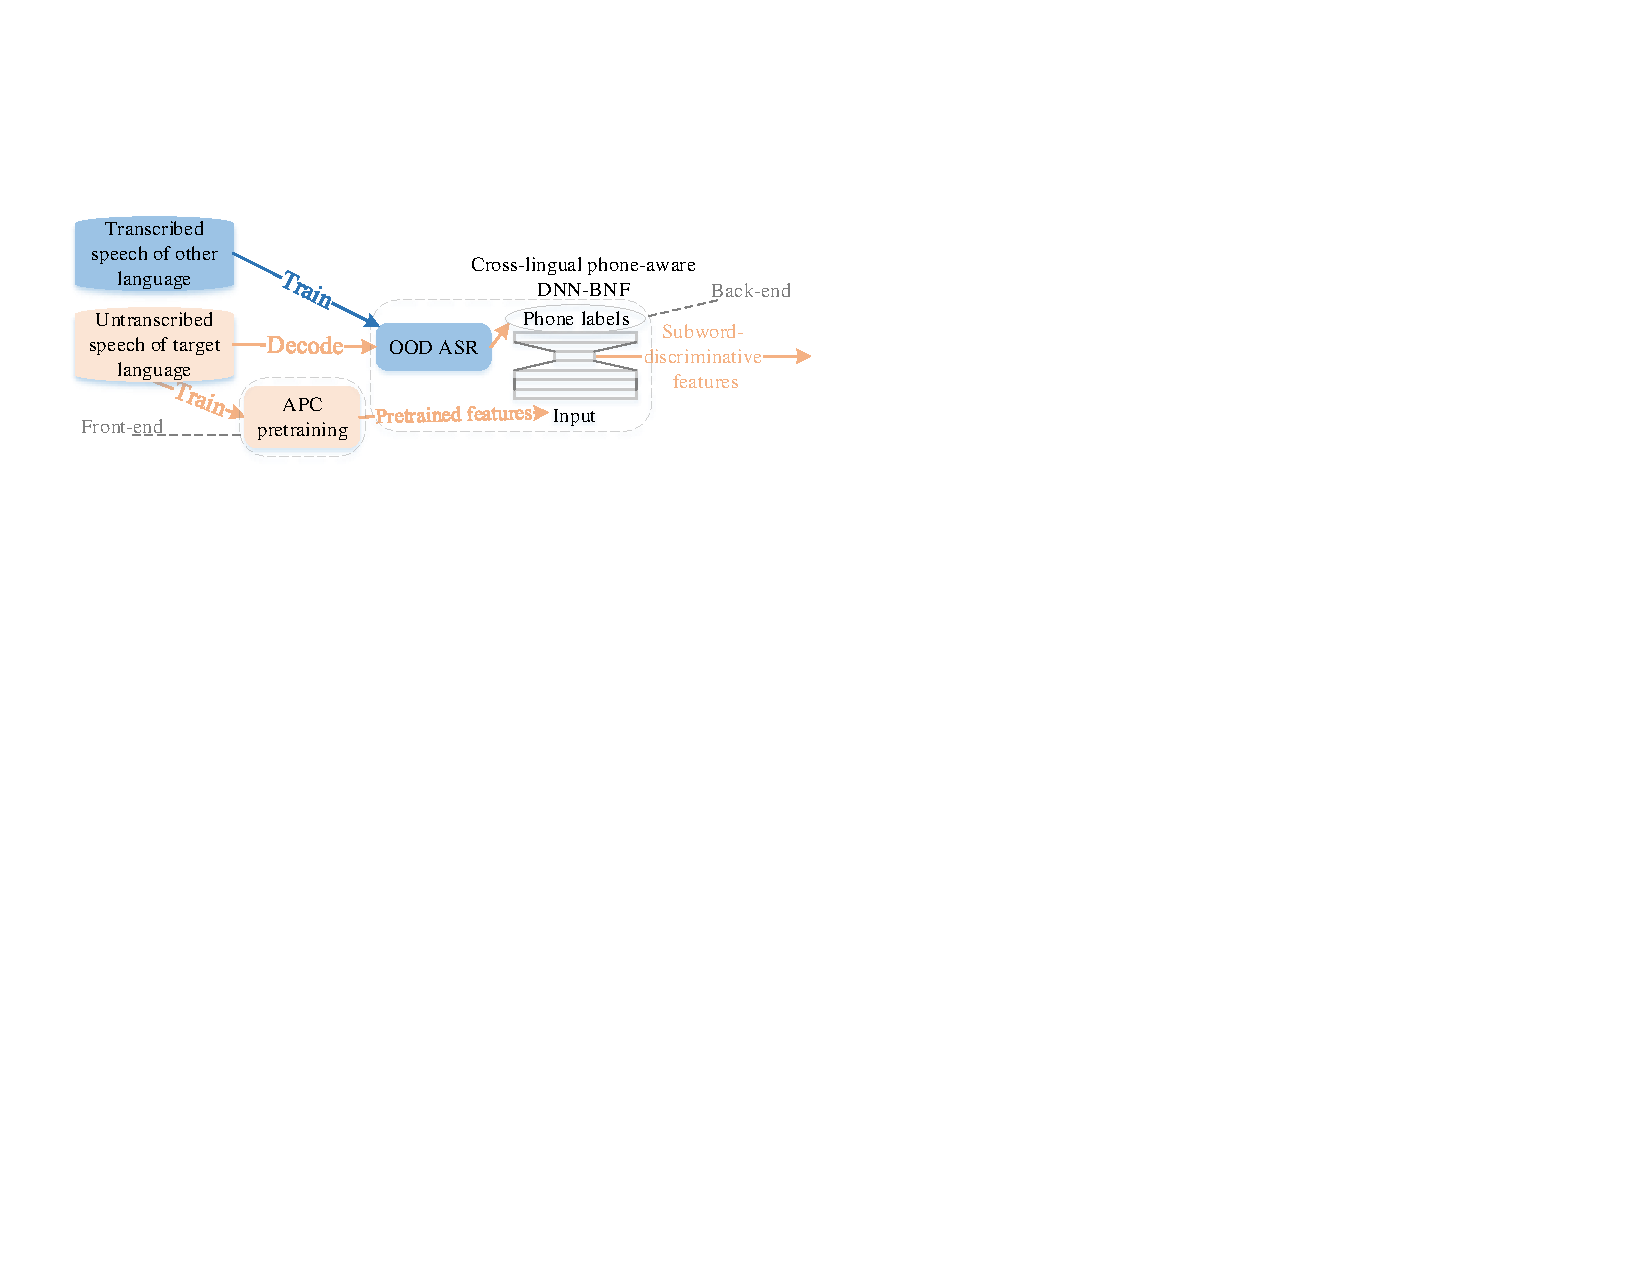
\includegraphics[width=\linewidth]{LaTeX/apc_framework_detail_other_lang.pdf}
    \caption{General framework of the proposed approach to unsupervised subword modeling.  }
    \label{fig:general_framework}
\end{figure}
The general framework of our proposed approach is illustrated in Figure \ref{fig:general_framework}. Given untranscribed speech data of a  target  language, an APC  model is pretrained in the front-end.
% stage.
% and used to extract pretrained features.
% is used to pretrain the data 
Next, an OOD ASR system trained on a language different from the target language  assigns a phone label to every frame of the target language's speech data through decoding. Pretrained features  created by the APC model and the cross-lingual phone labels created by the OOD ASR are then used to train a DNN-BNF model in the back-end, from which BNFs are extracted as the subword-discriminative representation in the final step.

% {\color{blue}
Front-end APC pretraining will be compared with an FHVAE approach \cite{hsu2017nips} which was used in related previous work \cite{Feng2019improving}. The whole pipeline of our approach will be compared with a system consisting of only the back-end DNN-BNF model, and a CPC approach \cite{oord2018cpc} applied in the same task \cite{kahn2019librilight}.
% , but without front-end APC pretraining.
Moreover, two different languages will be used to train two different OOD ASR systems for comparison.
% }
\subsection{APC pretraining}
\label{subsec:apc}
% APC is an unsupervised  feature representation learning method  with applications to various downstream tasks \cite{Chung2019}. 
% It was proposed by \cite{Chung2019} to learn frame-level feature representation which facilitates a wide range of downstream tasks. 
% The effectiveness of unsupervised APC pretraining  has been demonstrated in   ASR and speaker verification (SV) tasks \cite{Chung2019}. This  indicates that APC pretrained features could preserve both phonetic (subword) and speaker information from the original speech signal, meanwhile the two types of information are more  separable  to task-specific back-ends, comparing to spectral features and features learned by other methods \cite{Chung2019}. 
% In other words, 
In our concerned task, previously adopted feature learning methods 
% such as FHVAE \cite{Feng2019improving} and adversarial training \cite{Higuchi2019} 
usually target suppressing speaker variation, such as FHVAE \cite{Feng2019improving} and speaker adaptation \cite{heck2017feature}. In contrast, 
APC aims at learning
% the present study applies APC to learn 
a representation that keeps information from speech, while phonetic information is made more separable from speaker information. The learned representation is considered less risky of losing phonetic information than 
% {\color{blue}
  representations learned by methods in \cite{Feng2019improving,heck2017feature}.
% }
% expected to facilitate back-end subword-discriminative modeling, and is less risky of losing subword information.


% both subword and speaker information and they are more separable, hence facilitates back-end modeling to learn subword-discriminative representation of speech.%,  %The present study adopts APC to learn a feature representation

Let us assume a set of unlabeled speech frames $\{\bm{x_1}, \bm{x_2}, \ldots, \bm{x_T}\}$ for training, where $T$ is the total number of frames. At each time step $t$, the encoder of APC model $\textrm{Enc} (\cdot)$ reads as input  a feature vector 
$\bm{x_t}$, 
% $\bm{x_{1:t}}=\{\bm{x_1},\ldots,\bm{x_t}\}$ 
and outputs  a feature vector  $\bm{\hat{x}_t}$ (same dimension as $\bm{x_t}$) based on all the previous inputs $\bm{x_{1:t}}=\{\bm{x_1},\ldots,\bm{x_t}\}$,
\begin{equation}
    \bm{\hat{x}_t} = \textrm{Enc} (\bm{x_{1:t}}).
    \label{eqt:enc}
\end{equation}
The goal of APC is to let $\bm{\hat{x}_t}$ be as close as possible to $\bm{x_{t+n}}$, where $n$ is a pre-defined constant positive integer, denoted as \textit{prediction step}. 
% In other words, an APC tries to predict a speech frame that is $n$ steps ahead of the current time. 
The loss function during APC   training is defined as: $\textrm{Loss} = \sum_{t=1}^{T-n} \left| \bm{\hat{x}_t} - \bm{x_{t+n}} \right|$.
% \begin{equation}
%     \textrm{Loss} = \sum_{t=1}^{T-n} \left| \bm{\hat{x}_t} - \bm{x_{t+n}} \right|.
%     \label{eqt:apc_loss}
% \end{equation}
% By minimizing the loss function in Equation (\ref{eqt:apc_loss}), the APC encoder can be trained.
Intuitively, increasing $n$ encourages the   encoder to capture contextual dependencies in speech, 
% more global structures in speech, 
while a small $n$ focuses more on local smoothness.
 
Here, the encoder of APC $\mathrm{Enc} (\cdot)$ is realized by a long short-term memory (LSTM) \cite{hochreiter1997long} RNN. Let $L$ denote the number of LSTM layers,  Equation (\ref{eqt:enc}) is formulated as,
\begin{align}
    \bm{h_0} &= \bm{x_{1:t}},    \\
    \bm{h_l} &= \textrm{LSTM}^l (\bm{h_{l-1}}), l\in \{1,2,\ldots, L\}, \\
    \bm{\hat{x}_t} &= \bm{W} \bm{h_L},
\end{align}
where $\bm{W}$ is a trainable projection matrix. The equations that form  $\textrm{LSTM} (\cdot)$ can be found in \cite{sak2014long}. 

After APC training, the output of the top hidden layer $\bm{h_L}$ is extracted as the  learned acoustic representation, and is henceforth referred to as the  \textit{APC feature}. 
Although in principle,  $\bm{h_l}$ of any layer $l$ could be used as the learned representation, 
we follow \cite{Chung2019} in using the output of the top layer as they showed that this gave the best results in phone classification tasks.
% Results in \cite{Chung2019} suggest that outputs of higher layers  are more suitable for phone classification than lower layers. Following \cite{Chung2019} we choose to use the output of the top layer.
% , while lower layer outputs are  more suitable for speaker classification.
% Here $\bm{h_l}$ denotes the output of  

% , APC pretrained features surpass spectral features 
% which require 
% phonetic and speaker information in APC features are both more accessible to their respective back-end models for ASR and SV tasks.
% (-) Architecture of Enc.\\
% (-) how to extract features from APC to back-end.
% APC pretrained features  tend to retain as much information encoded in original speech representation as  possible. 
% different types of information in APC features, such as phonetic and speaker information, are both more accessible to the back-end models corresponding to their respective tasks.
\subsection{Cross-lingual phone-aware DNN-BNF}
% The back-end of our proposed approaches is t
% The DNN-BNF model  \cite{chen2017multilingual,feng2018exploiting} is adopted as the back-end of our proposed approach. 
As shown in Figure \ref{fig:general_framework}, the DNN-BNF back-end
% it 
is a DNN with a bottleneck   layer in the middle \cite{grezl2009investigation}. 
% BNFs could provide compact and subword-discriminative representation  \cite{grezl2009investigation}.  
% % Training of a subword-discriminative DNN-BNF model requires frame labels \cite{chen2017multilingual}. 
% In the zero-resource scenario, phone labels  required for DNN-BNF modeling are not directly available.
% Cross-lingual phone labels are utilized to train the DNN-BNF model.
% cannot be obtained due to the absence of transcriptions. 
% This study leverages an OOD  ASR system to generate cross-lingual phone labels for target  speech.
% {\color{blue}The motivation  is that
% % Although languages vary greatly in pronunciation, 
% speech sounds in different languages are believed to have much overlap at phone level.}
To obtain cross-lingual phone labels, the OOD ASR is used to decode  target speech utterances into  lattices,  and find the best path for every utterance. Afterwards, each speech frame is assigned with a triphone HMM state modeled by the OOD ASR. These   state labels provide phonetic representation for the target speech from a cross-lingual perspective. %They are denoted as cross-lingual phone labels.

% It is worth noting that decoding results depend on the relative weighting  of the ASR AM and language model (LM). In this study, the LM carries a very small weight, in order to ensure decoding results mainly reflect acoustic characteristics of target speech.

After obtaining triphone HMM state labels  as cross-lingual phone labels, the DNN-BNF  is trained using the pretrained APC features and the cross-lingual phone labels in a supervised manner \cite{grezl2007probabilistic}, and used to  extract BNFs   as the desired subword-discriminative feature representation. 
% BNFs are generated from the output of the bottleneck layer in the DNN-BNF model.
% The cross-lingual HMM labels are used as supervision for in-domain speech data in DNN-BNF modeling.
% After obtaining cross-lingual  HMM state labels, a DNN-BNF model is trained with target speech, using these labels as supervision.  
% The DNN-BNF is trained to optimize cross-lingual phone classification accuracy.
%The input features to DNN-BNF are APC features. 
% After training, the DNN-BNF is used to extract BNFs for target speech as the subword-discriminative feature representation. 
% The choice of languages to train the OOD ASR systems is flexible. 
% In the present study, OOD ASR systems for two different languages are utilized to generate the phone labels 
% {\color{blue}
% and learn two BNF representations. 
% Effectiveness of  the two  BNF representations  are compared.%  in the experiments.
% }
% to generate cross-lingual labels, in order to study the effect  of OOD  language identities on unsupervised subword modeling.
% its influence towards the final performance.
% our proposed approaches.

% (-) OOD ASR decoding\\
% (-) DNN-BNF training with APC features and cross-lingual phone labels\\
% (-) Effect of OOD language identity.
% Authors should observe the following rules for page layout. A highly recommended way to meet these requirements is to use a given template (Microsoft Word?? or LaTeX) and check details against the corresponding example PDF file. Given templates, Microsoft Word\textregistered\ or \LaTeX, can be adapted/imported easily in other software such as LibreOffice, Apple Pages, Lua\LaTeX, and Xe\LaTeX, but please be careful to match the layout of the provided PDF example.

\section{Experimental setup}

\subsection{Databases and evaluation metric}
% {\color{blue}
 English is chosen as the target language while Dutch and Mandarin are chosen as the two OOD languages. %.}
Training data for APC pretraining and DNN-BNF model training are taken from  Libri-light \cite{kahn2019librilight}, 
% Experiments in this study are carried out on two databases: Libri-light \cite{kahn2019librilight} and ZeroSpeech 2017 \cite{dunbar2017zero}. 
% Libri-light is 
a newly published English database
% and  by far the largest public database 
to support unsupervised subword modeling. 
% It is an English database.
% The language in Libri-light is English. 
The \textit{unlab-600} and  \textit{unlab-6K} sets from Libri-light are adopted. Unlab-600 is used in both APC pretraining and DNN-BNF model training, while unlab-6K is used only in DNN-BNF model training.
Unlab-600   consists of 
% $36,229$ utterances by $489$ speakers, summing up to
$526$ hours of speech excluding silence.
% non-silent speech. 
Additionally, we randomly select four subsets of utterances from unlab-600 to investigate the robustness of our approach to different amounts of training material. These subsets consist of $900$ (i.e., $13$ hours), $3.6$K ($52$ hours), $7.2$K ($104$ hours), and $14.4$K ($209$ hours)   utterances. 
Unlab-6K  set consists of $5,273$ hours of
% non-silent 
speech excluding silence.  Details of the training sets are listed in Table \ref{tab:libri_light_data}.
\begin{table}[!t]
\renewcommand\arraystretch{0.9}
\centering
\caption{Libri-light training data and its subsets.}
\resizebox{  \linewidth}{!}{%
\begin{tabular}{l|c|c|cccc}      
% \hline      
\toprule
&unlab-6K& unlab-600 & \multicolumn{4}{c}{subsets of unlab-600} \\%sub14.4K & sub7.2K & sub3.6K & sub0.9K \\
%  & \multicolumn{3}{c|}{ Training} & Test \\
\midrule
\#utterances &$362,817$ &  $36,229$ & $14,400$ &$7,200$ &$3,600$ &$900$ \\
\#speakers & $1,742$ & $489$ & $438$ & $393$ & $351$ & $244$ \\
Hours  & $5,273$ &$526$& $209$ & $104$ & $52$ & $13$ \\
\bottomrule
\end{tabular}%
% \footnotetext{`speakers-R/-L' denotes speakers with rich/limited speech data}
}
\label{tab:libri_light_data}
\end{table}

% {\color{blue}
The Dutch and Mandarin corpora used for training the two OOD ASR systems are the Corpus Spoken Dutch (CGN) \cite{oostdijk2000spoken} and Aidatatang\_200zh \cite{aidatatang}, respectively. 
% CGN is a  speech corpus covering various speaking styles including conversations, read speech, and broadcast news (BN).
% Speech spoken by people in the Netherlands are used. 
The CGN   training and test data partition follows \cite{laurensw75cgn_kaldi}. Its training data contains $483$ hours of speech, covering speaking styles including conversational and read speech and broadcast news.
Aidatatang\_200zh is a read speech   corpus.
% is a   read speech corpus developed by \cite{aidatatang}. The training set 
Its training data contains $140$ hours of speech.   
% }
%In order to better compare our approach with previous research in this area, we also tested our approach on the Zerospeech

Evaluation data are taken from  Libri-light and ZeroSpeech 2017 \cite{dunbar2017zero}. 
 Libri-light evaluation sets consist of \textit{dev-clean, dev-other, test-clean} and \textit{test-other}, 
% They are identical to the sets in Librispeech
% % , a widely used  corpus for ASR 
% \cite{panayotov2015librispeech}. 
% {\color{blue}
with 
% dev-/test-clean
$*$-clean 
having higher recording quality and accents closer to US English than  
% dev-/test-other
$*$-other 
\cite{panayotov2015librispeech}.
% }
% {\color{blue}
They are used to evaluate the effectiveness of  both front-end pretrained features and  BNFs learned by the back-end.
% .}

% {\color{blue}
Evaluation on ZeroSpeech 2017 aims  to better compare our approach with previous research in this area.
% } 
% We use the
% Here, 
English evaluation data from ZeroSpeech 2017 are used to evaluate the effectiveness of BNFs learned by the the back-end. These data are organized into subsets of differing   lengths (1s, 10s \& 120s)  \cite{dunbar2017zero}.
% ZeroSpeech 2017 database is   used in our experiments only for   performance evaluation purpose, 
% {\color{blue}
%They are used to evaluate the effectiveness of BNFs learned by the the back-end.
% } 
% English test data in ZeroSpeech 2017 is adopted, as our system regards English as the target language. 
% contains three languages, English, French and Mandarin. In our experiments, ZeroSpeech training data is not used, and 
% Our systems are trained solely on Libri-light. ZeroSpeech evaluation data for English is used. 

% consists of three utterance length settings, $1$s
% English 



The created BNFs, as well as APC pretrained features, are evaluated in terms of the ABX subword discriminability \cite{dunbar2017zero}.
In the ABX task, $A$, $B$ and $X$ are three speech segments, and $x$ and $y$ are two different phonemes. $A \in x$, $B \in y$, $X \in x$ or $y$. Following \cite{dunbar2017zero} (see also for more details), an error occurs if given a pre-defined distance measure $d$, $d(A,X) > d(B,X)$, given $X \in x$, 
or $d(A,X) < d(B,X)$, given $X \in y$.
% and vice versa.
% is to decide whether $X$ belongs to $x$ or $y$ if $A$ belongs to $x$ and $B$ belongs to $y$, where $A$, $B$ and $X$ are three speech segments, $x$ and $y$ are two different phonemes. 
% each consisting of $3$ consecutive phonemes (e.g. \quotes{b-e-g}). 
% $x$ and $y$ are two different phonemes. By saying $X$ belongs to $x$, it means the central phoneme in $X$ is $x$. 
%Details of  ABX error rate computation can be found in \cite{dunbar2017zero}, where 
Dynamic time warping is chosen as the distance measure. Segments $A$ and $B$   belong to the same speaker. ABX error rates for \textit{within-speaker} and \textit{across-speaker} are evaluated separately, depending
on whether X and A belong to the same speaker.
% A low ABX error rate is preferable as it indicates  the feature representation is good at distinguishing subword units. 
% Each pair of $A$ and $B$ are generated by the same speaker. 
% ABX error rates for \textit{within-speaker} and \textit{across-speaker} are evaluated separately, depending on whether $X$ and $A(B)$ belong to the same speaker. Software to compute ABX error rates on Libri-light and ZeroSpeech are both provided by their developers.

\subsection{Front-end}
% \subsection{APC and comparing method}
\label{subsec:exp_setup_apc_fhvae}
The APC model is implemented as a  multi-layer  LSTM network. Residual connections are made between two consecutive layers.  
Each LSTM layer has $100$ dimensions.
Unless specified explicitly, the number of LSTM layers is $3$.
% {\color{blue}
For each training data amount setting,
% } 
the
% The 
prediction step $n$ (in Section \ref{subsec:apc}) is
picked from $\{1,2,3,4,5\}$ which gives the best ABX performance.
% set to  the optimal value within $\{1,2,3,4,5\}$.
% , {\color{blue}one  for each training data amount setting.}
% different amounts of training material.} 
Our preliminary experiments showed that increasing $n$ to larger than $5$ would lead to rapid degradation in ABX error rate. 
The input features to APC are $13$-dimension MFCCs with cepstral mean normalization (CMN) at speaker level. 
The model is trained with the open-source tool by \cite{Chung2019} for $100$ epochs with the Adam optimizer \cite{kingma2014adam}, an initial learning rate of $10^{-4}$, and a batch size of $32$. 
%An open-source tool by \cite{Chung2019} is used to train the APC model. 
% MFCC features are extracted by Kaldi \cite{povey2011kaldi}. 
After training, the top LSTM layer's output is extracted as the APC feature representation.

% \color{blue}
The performance of front-end  APC pretraining is compared against FHVAE \cite{hsu2017nips}, which was used in related previous work \cite{Feng2019improving}. 
% As the reference model to compare the APC against, we use FHVAE \cite{hsu2017nips}.
% FHVAE was previously adopted \cite{Feng2019improving} as the front-end to address the same problem as in this study. 
The latent representation $\bm{z_1}$ of FHVAE is known to be preserving linguistic content while suppressing speaker variation \cite{hsu2017nips}, and is compared with the APC feature representation. The model architecture of FHVAE and its training procedure follow those in \cite{Feng2019improving}.
The FHVAE models are trained 
using an open-source tool \cite{hsu2017nips}, and take the same input features and training data (i.e., Libri-light) as the APC models. After training, the  FHVAE encoder's output $\bm{z_1}$ is extracted.
%The comparison is made 
 % Encoder structure, LSTM no. layers, input data size, $n$ is tuned. epochs, learning rate, batch size
\subsection{Back-end}
\subsubsection{OOD ASR systems}
\label{subsubsec:oodasr}
We trained two OOD ASR systems, i.e., a Dutch ASR and a Mandarin ASR.
% The Dutch ASR is trained with CGN \cite{oostdijk2000spoken}, while the Mandarin ASR is trained with Aidatatang\_200zh.
% , a transcribed speech corpus covering  speaking styles including conversations, read speech, broadcast news (BN), etc.
% % Speech spoken by people in the Netherlands are used. 
% The training and test data partition follows \cite{laurensw75cgn_kaldi}. The training data comprises $483$
% hours of speech. 
The OOD ASR systems use a chain-time delay NN (TDNN) AM \cite{povey2016purely} trained using Kaldi \cite{povey2011kaldi}, containing $7$   layers.  The TDNN   is trained based on the lattice-free maximum mutual information (LF-MMI) criterion \cite{povey2016purely}.
For Dutch, the input features consist of $40$-dimension high-resolution (HR) MFCCs. For Mandarin, the input  features consist of HR MFCCs  appended by 
% $3$-dimension 
pitch features \cite{ghahremani2014pitch}. 
%  Training data are speed perturbed with scales $0.9, 1.0$ and $1.1$, making the actual  amount of training data tripled. 
Frame labels required for TDNN training are obtained by forced-alignment with a GMM-HMM AM trained beforehand. 
% The number of modeled Dutch phones is $81$ (including a silence phone).  The number of modeled Mandarin phones is $119$ (including a silence phone). 
 For both systems, a tri-gram LM is trained using training data transcriptions.

The Dutch ASR obtained a word error rate (WER) of $8.98\%$ on the CGN broadcast test set. 
% {\color{blue}
(This   WER could be improved upon by integrating an   RNN LM. However, as Dutch ASR performance is not the focus of this study, an RNN LM is not applied.)
% } 
The Mandarin ASR obtained a character error rate (CER) of $6.37\%$ on the Aidatatang\_200zh test set.
% {\color{blue} 
The two ASR systems are used to generate cross-lingual phone labels for Libri-light training speech frames.
% }% for subsequent DNN-BNF model training.}

% , a read speech corpus developed by \cite{aidatatang}. The training set comprises $140$ hours of speech. 
% A chain-TDNN AM is trained. 



%  ; Speech by people from the Netherlands are used; This corpus comprises conversations, interviews, lectures, debates, read speech and broadcast news. Training and test data partition follows \cite{laurensw75cgn_kaldi}
% Training: $483$ hours, chain model, 
% TDNN, layer structure, input features, $81$ modeled phones (including a silence phone), $3,488$ triphone HMM states.
% gives WER $8.98\%$ on broadcast news test set. 

% Mandarin ASR trained with Aidatatang\_200zh \cite{aidatatang}
% Training data contains $140$ hours speech, read speech, TDNN model, input is MFCC plus pitch, $119$ modeled phones (including a silence phone), $4,400$ triphone HMM states , CER $6.37\%$ on test set. 

\subsubsection{DNN-BNF setup}
% \subsection{DNN-BNF setup}
Two DNN-BNF models are trained, one taking the Dutch cross-lingual phone labels as training labels and one taking the Mandarin  phone labels as training labels. % Both models are trained on the Libri-light (English) acoustic training data. 
% The cross-lingual phone labels are obtained from the Dutch or Mandarin OOD ASR system. 
%One DNN-BNF model is trained with phone labels generated by the Dutch ASR, while the other DNN-BNF is trained with labels generated by the Mandarin ASR. To obtain Dutch or Mandarin frame labels,  HR MFCC features (and appended by pitch features if to obtain Mandarin labels) of Libri-light are extracted, and fed as input features to the Dutch/Mandarin ASR system for decoding. 
% In order to generate cross-lingual phone labels, the Dutch or Mandarin ASR system is utilized to decode Libri-light training data.
% Cross-lingual phone labels are generated via decoding Libri-light training data using the Dutch or Mandarin ASR.
% During decoding, the LM to AM weight ratio is set to $0.001$.
% The decoding results, i.e. word transcriptions,  are  forced-aligned by the Dutch/Mandarin AM to generate HMM state alignments.
% \footnote{Here \textit{alignment} is different from the `norm'. It contains alternative pronunciations. This is required by Kaldi chain model training.}
% by chain model training of DNN-BNF in Kaldi.} 
% as frame labels.

The DNN-BNF consists of $7$ feed-forward layers (FFLs). Each layer has $450$ dimensions except a $40$-dimension bottleneck layer, which is located below the top FFL. 
% second top. 
The DNN-BNF uses a chain model which is trained based on  the   LF-MMI criterion. 
The inputs to DNN-BNF are the APC  feature with its neighboring ($-3$ to $+3$) frames. 
% contextual splicing $\{0, \pm 1, \pm 2, \pm 3\}$.
% Training labels are either Dutch  or Mandarin frame labels. 
After DNN-BNF training, $40$-dimension  BNFs are extracted as the learned subword-discriminative representation and evaluated with the ABX task.
% of target speech. 

% and phonetic-alignments in Dutch/Mandarin. 
% One could directly obtain frame labels from phonetic-alignments. However we rely on transcriptions to be aligned by Dutch/Mandarin AM. Just for practical consideration, as DNN-BNF is under Kaldi nnet3 recipe, 
%[kaldi chain model numerator FST]Instead of enforcing a particular pronunciation of the training data, we use as our reference a lattice of alternative pronunciations of the training data, generated by a lattice-generating decoding procedure using an utterance-specific graph as the decoding graph. This generates all alignments of pronunciations that were within a beam of the best-scoring pronunciation.



For the purpose of   comparison, two more DNN-BNF models are  trained using the $40$-dimension HR MFCC with its neighboring ($-3$ to $+3$) frames as input features. One model takes the Dutch labels  and the other takes the Mandarin labels.
% conventional spectral features as input features. 
% % {\color{blue}It is also implemented in our experiments.} 
% In this case, the %only difference during training is that
% % DNN-BNF training keeps the same as mentioned above, except that 
% input features before contextual splicing are $40$-dimensional HR MFCCs. 
Other  training and model settings   are unchanged.
% with the same contextual splicing. 
After  training, BNFs are extracted and also evaluated with the ABX task.
% BNF representation is   extracted.
% as a reference.
% including cross-lingual phone labeling, and DNN-BNF training.

\section{Results and discussion}
\subsection{Effectiveness of APC features }
\label{subsec:results_apc}
% {\color{blue}

% }
In this subsection, the APC  features and FHVAE features in the front-end ($\bm{z_1}$)  are directly evaluated using the ABX task, without being modeled by the  DNN-BNF back-end. %The performance comparison is made at front-end.
ABX error rates ($\%$) of the APC     and   FHVAE features with respect to different hours of training data  are shown in Figure \ref{fig:apc_fhvae_mfcc}.
\begin{figure}[!t]
    \centering
    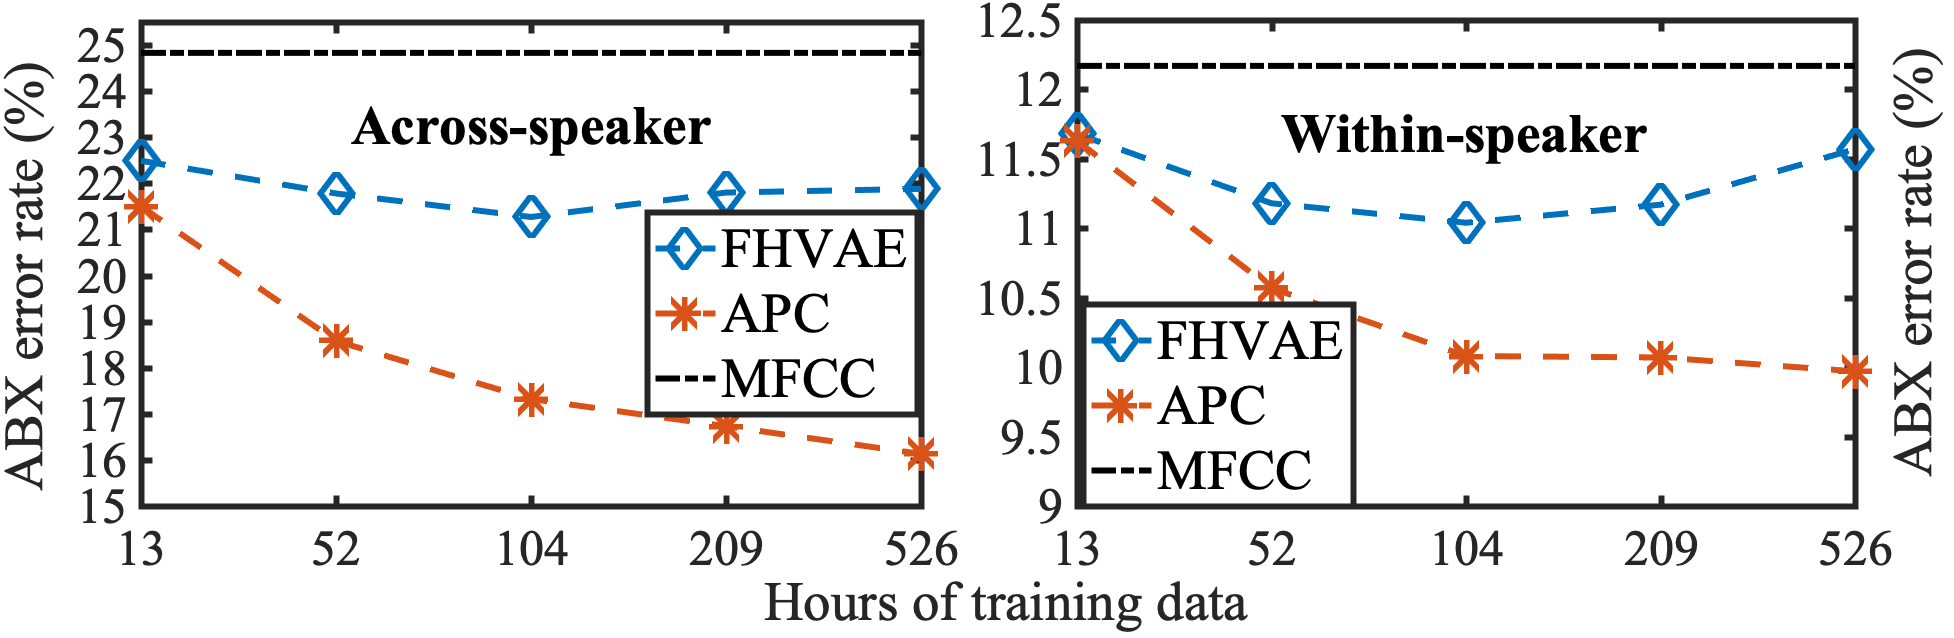
\includegraphics[width=1\linewidth]{LaTeX/apc_fhvae_mfcc_no_sub_hori_no_hrs.png}
    \caption{ABX error rates  of APC features, FHVAE features and official MFCC baseline on Libri-light (Avg. over $4$ sets). }
    \label{fig:apc_fhvae_mfcc}
\end{figure}
% these two features are learned without performing DNN-BNF modeling. 
ABX results in this figure are averaged values over the $4$ evaluation sets in Libri-light. The official MFCC baseline   \cite{kahn2019librilight} is also shown in this figure. It can be observed that both the APC features and the FHVAE features  outperform the MFCC features. The APC features are consistently superior to the FHVAE features in both the across- and the within-speaker conditions irrespective of the amount of training data.
Figure \ref{fig:apc_fhvae_mfcc} (left) indicates that the APC features are more robust to speaker variation than the FHVAE features, even though the APC model is not explicitly suppressing speaker variation as FHVAE is.
% , even though the
% % ($13 \sim 526$ hours, i.e. sub0.9K to unlab-600). 
% APC model is not explicitly suppressing speaker variation as FHVAE is.  
% Figure \ref{fig:apc_fhvae_mfcc} (left) indicates that APC features are more effective than   $\bm{z_1}$ in distinguishing subword units across different speakers.

% (-) a curve showing ABX error rate of APC features, FHVAE latent segment variables and MFCC features w.r.t training data amount.

\subsection{Effectiveness of BNF representation}
\label{subsec:results_bnf_librilight}
\begin{table}[!t]
\renewcommand\arraystretch{0.70}
\centering
\caption{ABX error rates of  BNFs, APC and CPC    on Libri-light.  Models are trained with unlab-600. APC   has $5$ layers, as this gives the best performance among different nos. of APC layers.}
\resizebox{1 \linewidth}{!}{%
\begin{tabular}{l|cc|cccc|c}      
% \hline      
\toprule
\midrule[0.2pt]
& \multicolumn{7}{c}{Across-speaker}\\
Feature&Input & Label & dev-clean & dev-other & test-clean & test-other & Avg.\\ 
\midrule
%  & \multicolumn{3}{c|}{ Training} & Test \\
\multirow{4}{*}{BNF} &APC & Du & $\bm{6.18}$&	$\bm{11.02}$&$	\bm{6.03}$	&$\bm{10.94}$&$	\bm{8.54}$\\
&MFCC & Du &$6.67$&$	11.65$&	$6.64$&$	12.00$&$	9.24$\\
&APC & Ma & $7.00$&$11.80$&$6.84$&$11.81$&$9.36$\\
% &APC & Ma & $6.89$&	$11.83$&	$6.82$&	$11.78	$&$9.33$\\
&MFCC & Ma & $7.92$&	$12.71$&	$7.74$&	$13.23$&	$10.40$\\
\midrule
APC& \multicolumn{2}{c|}{-} & $12.64$&$	19.00$&$12.19$&$18.75$&$15.65$\\
CPC \cite{kahn2019librilight} & \multicolumn{2}{c|}{-}&$9.58$&	$14.67$&	$9.00$&	$15.10$&	$12.09$\\
% \midrule


\midrule
&\multicolumn{7}{c}{Within-speaker} \\
% Input & Label & dev-clean & dev-other & test-clean & test-other & Avg.\\ 
\midrule
\multirow{4}{*}{BNF} &APC & Du  & $\bm{4.77}$&	$\bm{6.69}$&	$\bm{4.49}$&	$\bm{6.43}$&	$\bm{5.60}$\\
&MFCC & Du & $4.97	$&$6.94$&	$4.73$&	$6.86$&	$5.88$\\
&APC & Ma  & $5.25$&	$7.14$&	$5.21$&	$7.09$&	$6.17$\\
&MFCC & Ma & $6.06$&	$7.71$&	$5.62$&	$7.82$&	$6.80$\\
\midrule
APC&\multicolumn{2}{c|}{-}& $8.83$&$11.07$&$8.36$&$11.48$&$9.94$\\
CPC \cite{kahn2019librilight}&\multicolumn{2}{c|}{-} &$7.36$&	$9.39$&	$6.90$&	$9.59$&	$8.31$\\
% &dev-clean & dev-other & test-clean & test-other  \\
\midrule[0.2pt]
\bottomrule
\end{tabular}%

}
\label{tab:dnn_bnf}
\end{table}
In this subsection, all models are trained with unlab-600 ($526$ hours).
ABX error rates (\%) of BNFs extracted by the back-end DNN-BNF model are listed in Table \ref{tab:dnn_bnf}. The second and third columns  denote input feature types and frame labels for training DNN-BNF models. `Du' and `Ma' stand for Dutch and Mandarin. 
Two front-end features, i.e. APC and CPC (in \cite{kahn2019librilight}),  are also listed as references.
% {\color{blue}
% APC and CPC are   not modeled by the DNN-BNF back-end.
% Note that the APC model in Table \ref{tab:dnn_bnf} consists of $5$ LSTM layers instead of $3$. 
   From this table, it is observed  that:

(1) DNN-BNF trained with APC features performs better than that trained with MFCC features in all the evaluation sets. This  demonstrates the effectiveness of front-end APC pretraining in our proposed two-stage system framework.

(2) The BNFs obtained from the back-end DNN-BNF model outperform the APC features from the front-end. In other words, the results show that
% BNF outperforms the front-end APC  feature to a large margin. 
% The  BNF trained with  Dutch phone labels  achieves $45\%$ and $44\%$ relative error rate reduction over APC features in across- and within-speaker test conditions. 
% For DNN-BNF models trained with Mandarin labels, similar observation is   made. 
% The results show that 
back-end DNN-BNF modeling with cross-lingual phone labels
% leveraging OOD language resources 
outperforms front-end  pretrained features for unsupervised subword modeling, similar to what has been observed by \cite{shibata2017composite,feng2019_TASLP}. BNF also performs better than the   CPC feature    \cite{kahn2019librilight}. Note that CPC does not require OOD resources during training while BNF in this study does.

(3) The performance achieved by adopting Dutch labels in DNN-BNF model training is slightly better than that by adopting Mandarin labels. 
% ($9.33\%/6.17\%$). 
This can possibly be explained by the similarity between the OOD language and target in-domain language, i.e., Dutch and English, respectively, which are both West Germanic languages, while Mandarin is not. 
Although one could 
possibly 
attribute the superiority of adopting Dutch labels over Mandarin labels to the larger amount of training data for Dutch ($483$ hours) than for Mandarin ($140$ hours), this is not a likely explanation because both models achieved fairly similar 
% evaluation 
results 
% performance
on their respective in-domain test sets (in Section \ref{subsubsec:oodasr}).

% One may attribute the superiority of adopting Dutch labels over Mandarin ones to the larger amount of training data for the Dutch ASR ($483$ hours)  than that for the Mandarin ASR ($140$ hours).  
% % While the Dutch ASR  is trained with more data ($483$ hours) than the Mandarin ASR ($140$ hours), .
% In fact, evaluation results on their respective in-domain test sets (Dutch: $8.98\%$ WER; Mandarin: $6.37\%$ CER) indicate that the performance of the two OOD ASR systems do not differ much.

% their in-domain ASR performance (Dutch: $8.98\%$ WER; Mandarin: $6.37\%$ CER) do not differ much. 


%reveals the effect of the OOD language identity
% \begin{enumerate}
%     \item d
% \end{enumerate}

% (-) this part will give table to list results in detail. Table showing unlab-600 results. 

% Our proposed approaches best performance $8.54\%$ and $5.60\%$. 

% DNN-BNF with APC features better than that with MFCC features. 
% Mandarin labels slightly inferior to Dutch labels. 
% Probably is explained by language similarity English-Dutch is stronger than English-Mandarin. 
% Results better than CPC \cite{kahn2019librilight}, a purely unsupervised approach without leveraging OOD resources.

% (-) Need to mention in this part, APC encoder has $5$ LSTM layers instead of $3$.

% (-) May also draw observations between comparing Dutch labels and Mandarin labels. THen next subsection focuses on sensitivity of training data amount
% DNN-BNF trained with Dutch labels is discussed. Mandarin labels will be included in the next subsection. 

\subsection{Effect of amount of training data}
\begin{figure}[!t]
    \centering
    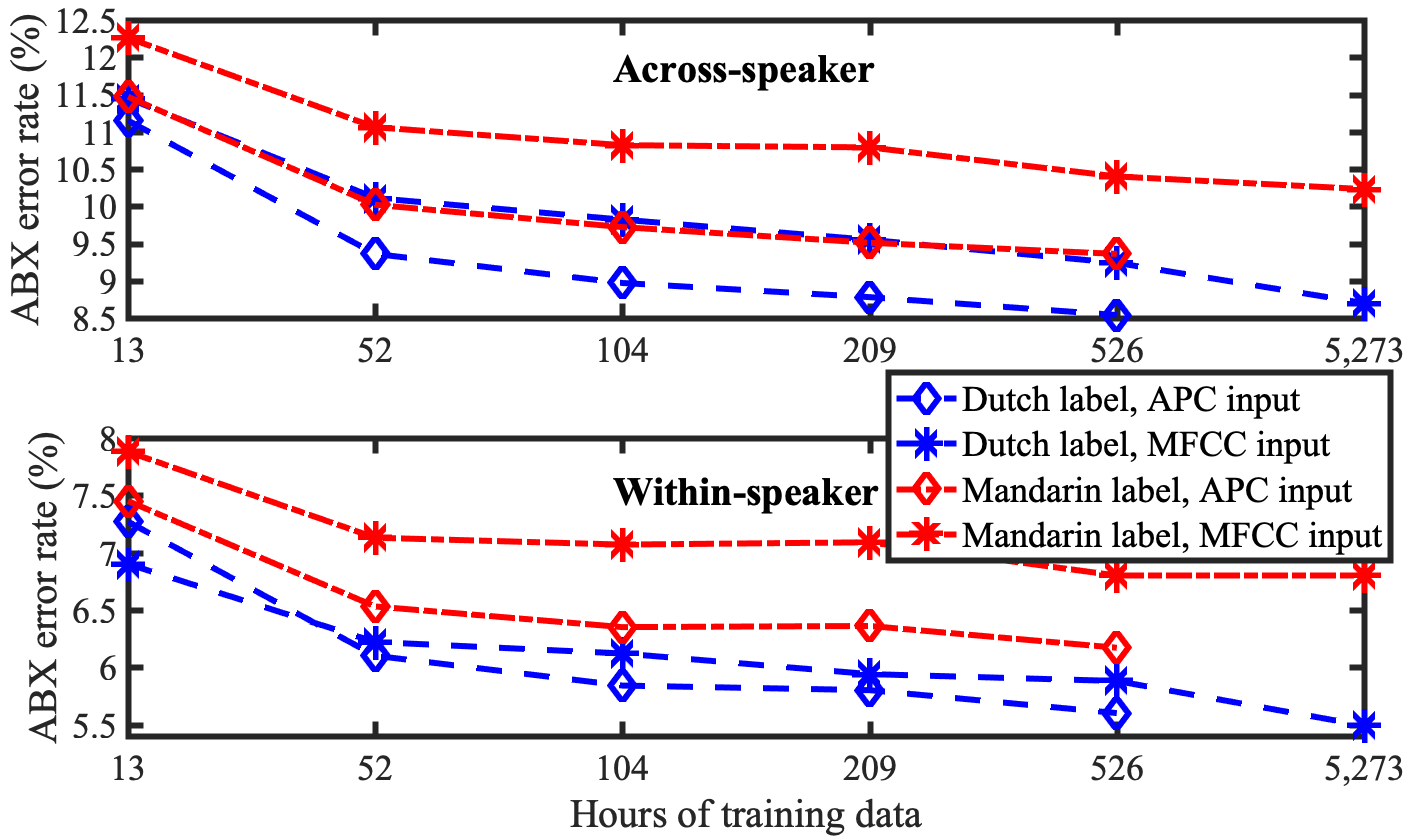
\includegraphics[width=0.9\linewidth]{LaTeX/crsling_dnn_bnf_apc_input_vert_no_prefix_adt_apc_across_9.36_hori_no_hrs.png}
    \caption{ABX error rates of BNFs w.r.t amount of training data on Libri-light (Avg. over $4$ sets).}
    \label{fig:dnn_bnf_data_amount}
\end{figure}

ABX error rates ($\%$) of BNFs extracted by  DNN-BNF models with respect to different amounts of training data in hours are illustrated in Figure \ref{fig:dnn_bnf_data_amount}. The results are averaged values over the $4$ evaluation sets in  Libri-light. Unlab-6K ($5,273$ hours)  is only adopted in training DNN-BNF models with MFCC input features (marked as ``$\ast$''). For models trained with APC features as input features (``$\diamond$''), the  data amount for APC pretraining and DNN-BNF model training   is the same for each run.  From Figure \ref{fig:dnn_bnf_data_amount}, it can clearly be seen that 
% increasing the amount of training data leads to better ABX performance. 
% When training data increases from $13$ hours to $52$ hours, 
performance improves as more training data is available, with the largest improvement when the training data increases from $13$  hours  to $52$ hours, and less improvement for any additional training material.
%compared to   that from $52$ hours to over $500$ hours. 

Secondly, across the different data amounts, the DNN-BNF models trained with APC features as input features are almost consistently better than those with MFCC input features. 
Interestingly, for Dutch, the model that uses APC features and is trained with $209$ hours of data achieves similar across-speaker error rates ($8.78\%$) to the model trained with MFCCs with $5,273$ hours of data ($8.70\%$). This implies that APC pretraining ``saves'' around $5,000$ hours (i.e.  $96\%$) of training data, making APC pretraining highly appealing in low-resource speech modeling. The effect of pretraining on the needed amount of training data is even larger when Mandarin labels are used for DNN-BNF modeling (saving over $99\%$ of the training data).
% $10.02\%$ across-speaker error rate is achieved using APC features and trained with $52$ hours of data, comparing to $10.23\%$ error rate achieved using MFCC features and trained with $5,273$ hours of data. 
%, APC pretraining  could save even more training data amount without ABX error rate degradation. 
% In real-world applications, it is sometimes impractical to gain knowledge on language similarity between the target unknown language and resource-rich languages. 
% APC pretraining 
% From this perspective,
% Mandarin phone labels are less ideal to English speech than Dutch ones, making DNN-BNF input feature quality more essential.
% The benefit of data increase is twofold: improvement on APC features
% This set comprises $5.3$K hours of speech, roughly tenfold of unlab-600.


% compare results of dnn-bnfs with Dutch ASR labels and Mandarin ASR labels.
% Will show as Figure  \ref{fig:dnn_bnf_data_amount}. 
% Will have to introduce unlab-6K set.
% Need to explain in Figure \ref{fig:dnn_bnf_data_amount}
% , for systems with APC features as input, the training set used in APC pretraining and DNN-BNF modeling is always the same.

% (-) Increasing from 10+ hours to 50+ hours gives prominent performance improvement. from 50+ hours to 500+ hours the improvement still there but more gradual.

% (-) By applying APC pretraining, DNN-BNF consistently outperform that w/o APC. Particularly most cases, w/ APC at 522h more effective than w/o APC but at 5.2K h.


% \section{Discussion}
\subsection{ZeroSpeech 2017 results}

% \begin{table}[!t]
% \renewcommand\arraystretch{0.50}
% \centering
% \caption{ABX error rates of  BNFs  on ZeroSpeech 2017 English sets. Models are trained with  Libri-light using Dutch labels.}
% \resizebox{1 \linewidth}{!}{%
% \begin{tabular}{cc|ccc|c|ccc|c}      
% % \hline      
% \toprule
% \midrule[0.2pt]
% & &\multicolumn{4}{c|}{Across-speaker}& \multicolumn{4}{c}{Within-speaker}\\
% System &   Train hrs & 1s & 10s & 120s & Avg. &1s &10s &120s &Avg.\\
% \midrule[0.2pt]

% \multirow{ 3}{*}{Proposed} & $526$  & $7.65$&$6.69$&$6.66$&$\bm{7.00}$&$5.52$&$4.77$&$4.68$&$\bm{4.99}$\\
% & $209$ & $8.11$&$6.99$&$6.90$&$7.33$&$5.83$&$5.06$&$4.97$&$5.29$\\
% & $104$ & $8.14$&$7.07$&$7.03$&$7.41$&$5.89$&$4.99$&$5.00$&$5.29$ \\
% \midrule[0.2pt]
% Topline \cite{dunbar2017zero}&  &$8.6$&$6.9$&$6.7$&$7.40$ &$6.5$&$5.3$&$5.1 $&$5.63$\\
%   \cite{shibata2017composite}& & $7.9$&$7.4$&$6.9$&$7.40$&$5.5$&$5.2$&$4.9$&$5.20$\\
% \midrule[0.2pt]
% \bottomrule
% \end{tabular}%
% }
% \label{tab:zrsc2017}
% \end{table}

\begin{table}[!t]
\renewcommand\arraystretch{0.70}
\centering
\caption{ABX error rates of  BNFs  on ZeroSpeech 2017 English evaluation sets. Models are trained with  Libri-light.}
\resizebox{1 \linewidth}{!}{%
\begin{tabular}{cc|ccc|c|ccc|c}      
% \hline      
\toprule
\midrule[0.2pt]
& &\multicolumn{4}{c|}{Across-speaker}& \multicolumn{4}{c}{Within-speaker}\\
System &   Hours &  1s & 10s & 120s & Avg. &1s &10s &120s &Avg.\\
\midrule[0.2pt]

\multirow{ 3}{*}{Proposed-Du} & $526$  &  $7.65$&$6.69$&$6.66$&$\bm{7.00}$&$5.52$&$4.77$&$4.68$&$\bm{4.99}$\\
& $209$&  $8.11$&$6.99$&$6.90$&$7.33$&$5.83$&$5.06$&$4.97$&$5.29$\\
& $104$&  $8.14$&$7.07$&$7.03$&$7.41$&$5.89$&$4.99$&$5.00$&$5.29$ \\
\midrule
\multirow{ 3}{*}{Proposed-Ma} 
& $526$  &  $8.19$&$7.33$&$7.30$&$7.61$&$5.97$&$5.39$&$5.37$&$5.58$ \\
& $209$& $8.62$&$7.61$&$7.52$&$7.92$&$6.31$&$5.52$&$5.60$&$5.81$\\
& $104$&   $8.47$&$7.62$&$7.52$&$7.87$&$6.13$&$5.49$&$5.44$&$5.69$\\
\midrule[0.2pt]
Topline \cite{dunbar2017zero}&  &$8.6$&$6.9$&$6.7$&$7.40$ &$6.5$&$5.3$&$5.1 $&$5.63$\\
  \cite{shibata2017composite}& & $7.9$&$7.4$&$6.9$&$7.40$&$5.5$&$5.2$&$4.9$&$5.20$\\
\midrule[0.2pt]
\bottomrule
\end{tabular}%
}
\label{tab:zrsc2017}
\end{table}
We also evaluated the performance of  our approach 
% by adopting Dutch (-Du) and Mandarin (-Ma) labels
% adopting Dutch labels
% \footnote{{\color{blue}Performance with Mandarin labels is not reported due to page limit.}} 
on the ZeroSpeech 2017 English evaluation sets. The results are shown in Table \ref{tab:zrsc2017}, which also includes the official topline \cite{dunbar2017zero}  and the best-performing system (using OOD data) \cite{shibata2017composite}. 
Note that, unlike our approach, these two systems employed English labeled data. 
The total amount of labeled training data used in \cite{shibata2017composite} is $1,327$ hours (including $80$-hour English data).
In this table, ``Proposed-Du/-Ma'' denotes our proposed approach by adopting Dutch or Mandarin labels  respectively.
Interestingly, using Dutch labels, our system trained with $526$ hours of data outperforms the topline and \cite{shibata2017composite} systems, and is comparable to the two reference systems when trained with only $104$ hours of data. Table \ref{tab:zrsc2017} also shows the proposed approach by adopting Dutch labels performs better than that by adopting Mandarin labels,  which is consistent with observations in Section \ref{subsec:results_bnf_librilight}.

% The system \cite{shibata2017composite} is best-performing.

% report our results and 
% supervised topline, as well as 
% recent papers benchmarked here, \cite{riviere2020unsupervised} used Librispeech-360 to train CPC;
% \cite{shibata2017composite} best system used 10 languages including English labeled data; 
% \cite{chorowski2019unsupervised} used ZRSC training data only.

\section{Conclusions}
This study addresses unsupervised subword modeling, and proposes a two-stage system that consists of APC pretraining and cross-lingual phone-aware DNN-BNF modeling.  
% Experiments are carried out on Libri-light and ZeroSpeech 2017 databases and evaluated by the ABX task. 
Experimental results on Libri-light and ZeroSpeech 2017 databases demonstrate the effectiveness of APC in front-end feature pretraining. It surpasses a previously adopted FHVAE approach. Our whole system outperforms the state of the art on both databases. 
Cross-lingual phone labeling for English data by a Dutch ASR is slightly better than by a Mandarin ASR. This is possibly linked to the larger similarity of Dutch than Mandarin with  English.  
The proposed approach benefits from increasing training data amount, and is less sensitive to data amount when the training data is over $50$ hours. 
% {\color{blue}
When using APC pretraining, $4\%$ of the training material could result in a similar   performance to   using the full training set without  APC pretraining.
% }
% APC pretraining could save the amount of training data from over $5,000$ hours to around $200$ hours for the proposed system with little performance degradation in across-speaker ABX error rate.  

% \section{Acknowledgements}




\bibliographystyle{IEEEtran}

\bibliography{mybib}

% \begin{thebibliography}{9}
% \bibitem[1]{Davis80-COP}
%   S.\ B.\ Davis and P.\ Mermelstein,
%   ``Comparison of parametric representation for monosyllabic word recognition in continuously spoken sentences,''
%   \textit{IEEE Transactions on Acoustics, Speech and Signal Processing}, vol.~28, no.~4, pp.~357--366, 1980.
% \bibitem[2]{Rabiner89-ATO}
%   L.\ R.\ Rabiner,
%   ``A tutorial on hidden Markov models and selected applications in speech recognition,''
%   \textit{Proceedings of the IEEE}, vol.~77, no.~2, pp.~257-286, 1989.
% \bibitem[3]{Hastie09-TEO}
%   T.\ Hastie, R.\ Tibshirani, and J.\ Friedman,
%   \textit{The Elements of Statistical Learning -- Data Mining, Inference, and Prediction}.
%   New York: Springer, 2009.
% \bibitem[4]{YourName17-XXX}
%   F.\ Lastname1, F.\ Lastname2, and F.\ Lastname3,
%   ``Title of your INTERSPEECH 2020 publication,''
%   in \textit{Interspeech 2020 -- 20\textsuperscript{th} Annual Conference of the International Speech Communication Association, September 15-19, Graz, Austria, Proceedings, Proceedings}, 2020, pp.~100--104.
% \end{thebibliography}

\end{document}
